\subsection{Rapid Miner} % (fold)
\label{sub:Rapid Miner}
Our tool of choice was Rapid Miner because 
 GUI interface is very user friendly and it wraps a far more 
implementations of data mining algorithms than Weka. In fact, it contains Weka too.

    Apart from interface it works flawlessly and it also contains presenting features e.g. diagrams, graphs, etc.

The pictures below shows the GUI interface of Rapid Miner
and the pictures presents workflow of our experiments.
In each of our experiment included the experiments with weka we went through the phases of loading data, preprocess it, choose label attribute, use cross validation. The cross validation steps is depicted in detail in next picture and it itself contains phases of training the model and testing it.

\begin{figure}[!hbp]
\begin{center}
    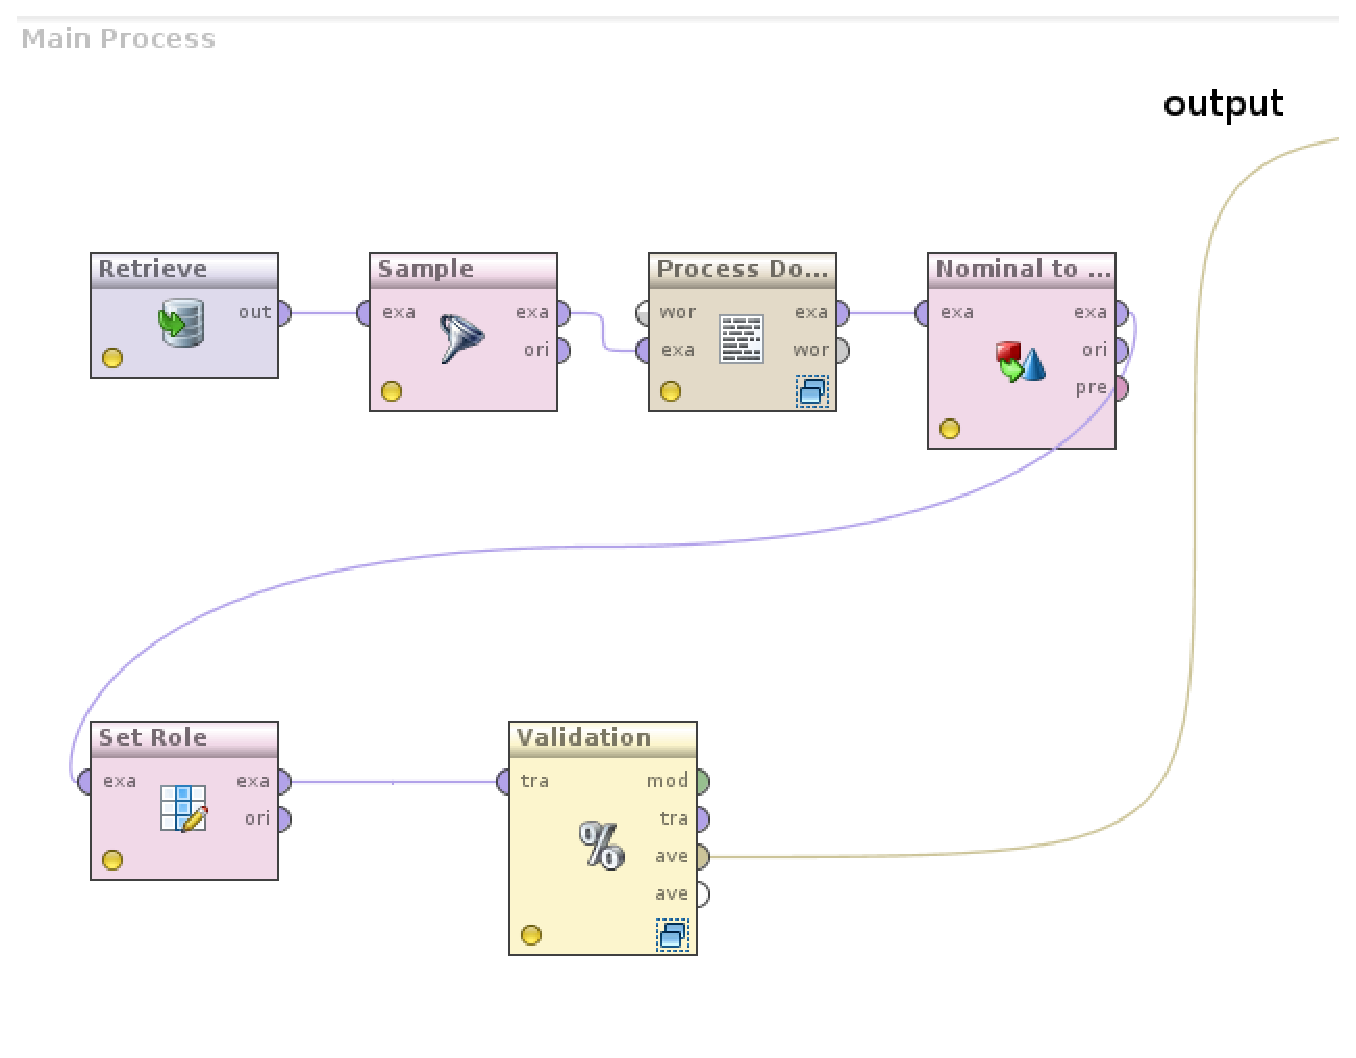
\includegraphics[scale=0.5]{rapidMiner-process}
\caption{\label{pic:st_art}  Rapid Miner Experiment worklow}
\end{center}
\end{figure}

\begin{figure}[!hbp]
\begin{center}
    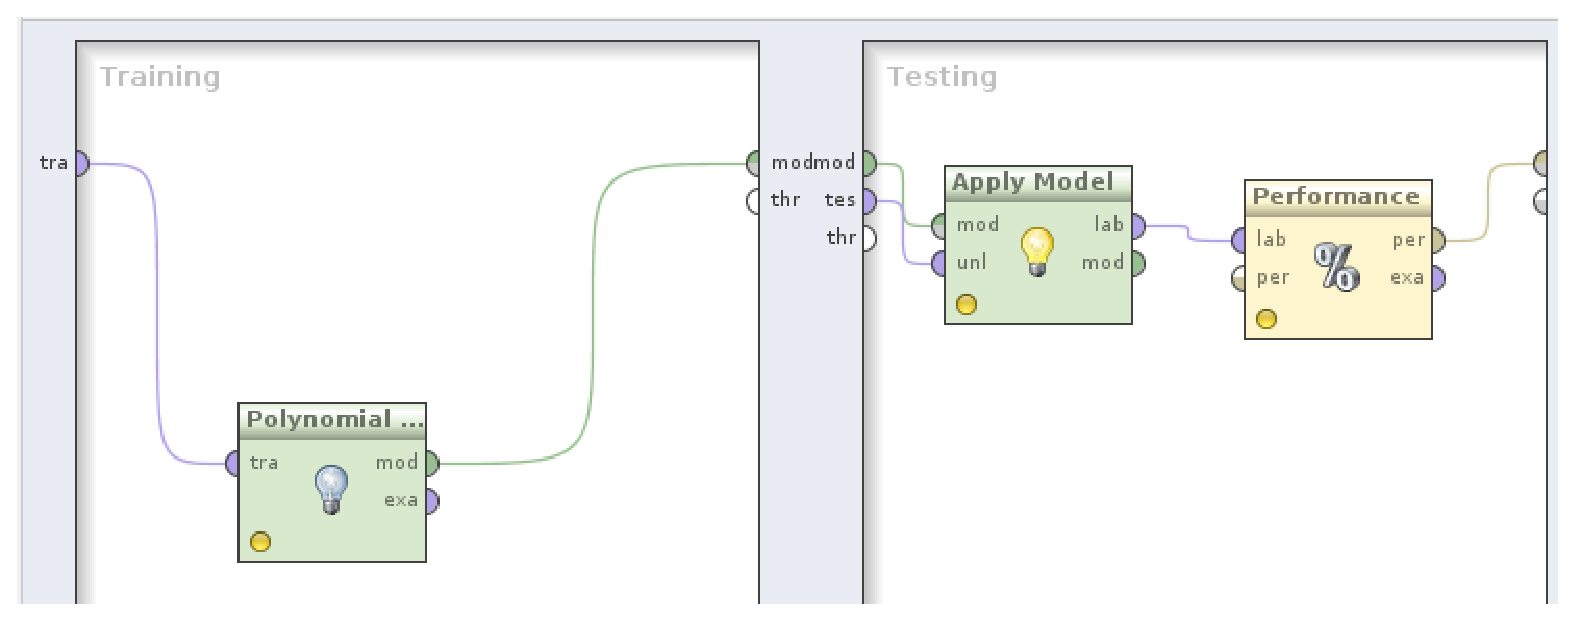
\includegraphics[scale=0.5]{rapidMiner-process-validation}
\caption{\label{pic:st_art}  Cross Validation Rapid miner visualisation}
\end{center}
\end{figure}

end{figure}

% subsection Rapid Miner (end)
